% Figure s10f02_nnqs (Session 10): neural network quantum states.
% The image is rendered by figures/blender/s10f02_nnqs.py; the coordinates of the labels come from
% figures/blender/out/s10f02_nnqs*_anchors.tex. Build with figures/blender/build_figure.sh s10f02_nnqs.
\documentclass[11pt,tikz,border=0pt]{standalone}
\usepackage[T1]{fontenc}
\usepackage{amsmath,amssymb,graphicx,bm}
\usepackage{xcolor}
\usetikzlibrary{arrows.meta,calc}
% The three label colors of the figures, with the same values as in src/figures_preamble.tex.
\definecolor{aqmaccent}{RGB}{31,78,121}
\definecolor{aqmbroken}{RGB}{168,42,34}
\definecolor{aqmmuted}{RGB}{125,125,125}

% Shared TikZ styles of the overlays: axis arrows drawn on top of the renders, between anchors
% written by the scripts, so that they can be adjusted without rendering again.
\tikzset{
  axarrow/.style={line width=0.6pt, draw=black!70, -{Stealth[length=4.5pt,width=3.5pt]}},
  axlbl/.style={font=\small, inner sep=1.5pt},
}
% A discrete color key: \aqmkey{(x,y)}{color 1}{label 1}{color 2}{label 2} draws two swatches in a
% column with their labels, anchored at its north west corner. The colors are the sRGB values
% used in the render, defined below.
\definecolor{keypos}{RGB}{118,158,198}
\definecolor{keyneg}{RGB}{214,150,132}
\definecolor{keyup}{RGB}{224,62,40}
\definecolor{keydown}{RGB}{40,92,200}
\definecolor{keydark}{RGB}{31,78,121}
\definecolor{keylight}{RGB}{118,158,198}
\newcommand{\aqmkey}[5]{%
  \begin{scope}[shift={#1}]
    \fill[#2, draw=black!40, line width=0.3pt] (0,-0.32) rectangle (0.32,0);
    \node[font=\small, anchor=west, inner sep=1.5pt] at (0.38,-0.16) {#3};
    \fill[#4, draw=black!40, line width=0.3pt] (0,-0.74) rectangle (0.32,-0.42);
    \node[font=\small, anchor=west, inner sep=1.5pt] at (0.38,-0.58) {#5};
  \end{scope}}
% The same key in one row, for a figure with no room for a column.
\newcommand{\aqmkeyrow}[5]{%
  \begin{scope}[shift={#1}]
    \fill[#2, draw=black!40, line width=0.3pt] (0,-0.32) rectangle (0.32,0);
    \node[font=\small, anchor=west, inner sep=1.5pt] (k1) at (0.38,-0.16) {#3};
    \fill[#4, draw=black!40, line width=0.3pt] ([xshift=0.25cm]k1.east |- 0,-0.32) rectangle ++(0.32,0.32);
    \node[font=\small, anchor=west, inner sep=1.5pt] at ([xshift=0.63cm]k1.east) {#5};
  \end{scope}}

\newlength{\figw}\setlength{\figw}{15.60cm}   % the text width of the notes (A4, 2.7 cm margins)

\begin{document}
\begin{tikzpicture}[lbl/.style={font=\small, inner sep=1.5pt}, pnl/.style={font=\small\bfseries, inner sep=1.5pt}]
  \begin{scope}[shift={(0.00cm,0.00cm)}]
    \setlength{\figw}{15.60cm}
    \node[anchor=south west, inner sep=0pt] at (0,0)
      {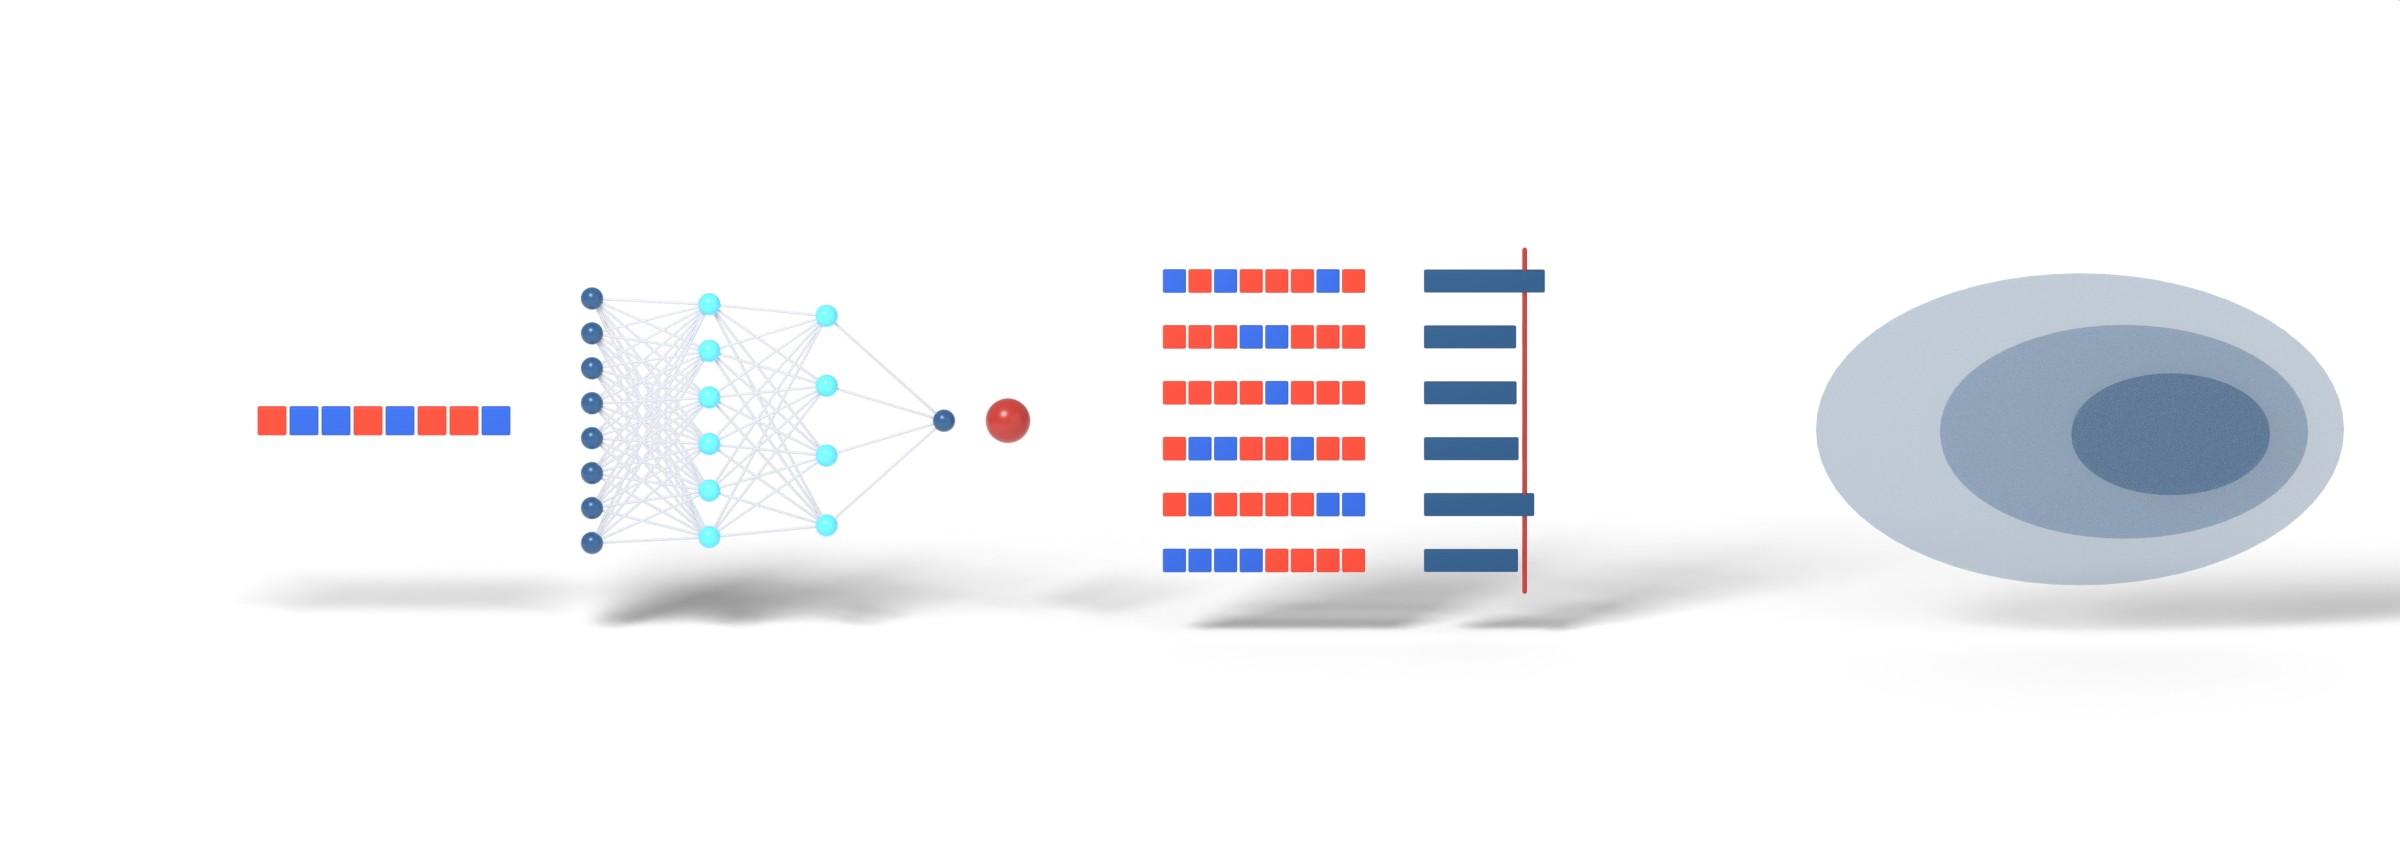
\includegraphics[width=\figw]{../blender/out/s10f02_nnqs.jpg}};
    %% written by figlib.py; x and y in units of the image width
\coordinate (as) at (0.1600\figw,0.1624\figw);
\coordinate (aC) at (0.4200\figw,0.1979\figw);
\coordinate (ap) at (0.1000\figw,0.2594\figw);
\coordinate (bs) at (0.5267\figw,0.1074\figw);
\coordinate (be) at (0.6353\figw,0.2562\figw);
\coordinate (bp) at (0.4733\figw,0.2594\figw);
\coordinate (nnqs) at (0.9272\figw,0.2381\figw);
\coordinate (peps) at (0.9272\figw,0.2174\figw);
\coordinate (mps) at (0.9272\figw,0.1979\figw);
\coordinate (cp) at (0.7467\figw,0.2594\figw);

    \node[pnl, anchor=south west] at (ap) {(a)};
    \node[pnl, anchor=south west] at (bp) {(b)};
    \node[pnl, anchor=south west] at (cp) {(c)};
    \node[lbl, anchor=north] at (as) {configuration $s$};
    \node[lbl, anchor=south, text=aqmbroken] at (aC) {$C_\theta(s)$};
    \node[lbl, anchor=north] at (bs) {samples from $|C_\theta(s)|^2$};
    \node[lbl, anchor=south, text=aqmbroken] at (be) {$\langle E_{\rm loc}\rangle$};
    \node[lbl, anchor=north] at (nnqs) {NNQS};
    \node[lbl, anchor=north] at (peps) {PEPS};
    \node[lbl, anchor=north, text=white] at (mps) {MPS};
    \aqmkeyrow{(4.6cm,0.55cm)}{keyup}{$\uparrow$}{keydown}{$\downarrow$}
  \end{scope}
\end{tikzpicture}
\end{document}
